% This is a template for Ph.D. dissertations in the UCI format.

% All fonts, including those for sub- and superscripts, must be 10 points or larger.
% Recommended sizes are 14-point for chapter headings, 12-point for the main body of text
% and figure/table titles, and 10-point for footnotes, sub- and super-scripts, and text in
% figures and tables.
\documentclass[12pt,fleqn]{ucithesis}

\usepackage{amsmath}
\usepackage{array}
\usepackage{bm}
\usepackage{boxedminipage}
\usepackage{graphicx}
%\usepackage{natbib}
%http://merkel.zoneo.net/Latex/natbib.php
\usepackage[numbers]{natbib}
\usepackage{path}
\usepackage{psfrag}
\usepackage{relsize}
%\usepackage{subfigure}
%\usepackage{subfig}
\usepackage{todonotes}
\usepackage{bytefield}
\usepackage{url}
\usepackage{verbatim}
\usepackage{caption}
\usepackage{subcaption}
\usepackage{listings}

% plainpages=false fixes the "duplicate ignored" error with page counters
% Set pdfborder to 0 0 0 to disable colored borders around PDF hyperlinks
\usepackage[plainpages=false,pdfborder={0 0 0}]{hyperref}



\graphicspath{{figures/}}

% Uncomment the following line to enable Unicode support. This will allow you
% to enter non-ASCII characters (such as accented characters) directly without
% having to use LaTeX's awkward escape syntax (e.g., \'{e})
% NOTE: You may have to install the ucs.sty package for this to work. See:
% http://www.unruh.de/DniQ/latex/unicode/
% \usepackage[utf8x]{inputenc}

\begin{document}


\thesistitle
{
  Improving the Architecture of Calico
}

\degreename{Master of Science}

% Use the wording given in the official list of degrees awarded by UCI:
% http://www.rgs.uci.edu/grad/academic/degrees_offered.htm
\degreefield{Information and Computer Science}

% Your name as it appears on official UCI records.
\authorname{Mitchell Ryan Dempsey}

% Use the full name of each committee member.
\committeechair{Professor Andr\'{e} van der Hoek}
\othercommitteemembers
{
  Professor James A. Jones\\
  Professor Richard N. Taylor
}

\degreeyear{2012}

\copyrightdeclaration
{
  {\copyright} {\Degreeyear} \Authorname
}

% If you have previously published parts of your manuscript, you must list the
% copyright holders; see Section 3.2 of the UCI Thesis and Dissertation Manual.
% Otherwise, this section may be omitted.
% \prepublishedcopyrightdeclaration
% {
%   Chapter 4 {\copyright} 2003 Springer-Verlag \\
%   Portion of Chapter 5 {\copyright} 1999 John Wiley \& Sons, Inc. \\
%   All other materials {\copyright} {\Degreeyear} \Authorname
% }

% The dedication page is optional.
% \dedications
% {
%   To my parents...
% }

\acknowledgments
{
  I would like to thank my advisor, Professor Andr\'{e} van der Hoek. Without his help and guidance my thesis would not be possible.
  I want to thank the members of the Software Design and Collaboration Lab: Nick Mangano, Nicolas Lopez, Gerald Bortis, Alex Baker, Tiago Proenca, and Nilmax Moura. I truly enjoyed my time spent with them, and greatly appreciate the help they have provided over the years.
}

% max 250 words
\thesisabstract
{
  Calico is a software design sketching tool that aims to support software designers by helping them work through a design problem by sketching potential solutions. 
  Calico was designed to be used with an interactive whiteboard so that it can replicate the feel of a traditional whiteboard while at the same time enabling advanced functionality. 

  There were three main problems with the original version of Calico: 
  (1) distributed designers were not well supported, 
  (2) collaboration was not natively supported,
  and (3) it was very difficult to add new functionality.
  This thesis examines these problems and presents various solutions:
  (1) creating a performance-based network architecture,
  (2) centering Calico around collaboration,
  and (3) creating a plugin framework to easily add new functionality.

  Prior to this work, Calico was unable to meet the demands of designers in the field. By resolving these problems, Calico was able to be deployed both in-house in our design lab, as well as in Informatics 122 (a software design course).
}

\preliminarypages

\chapter{Introduction}

Software design tools offer the user a significant amount of power when it comes to tool support. 
Using these tools, designers can generate various design diagrams such as architecture diagrams, flowcharts, relational diagrams.
Tools have been created to support all forms of software design, ranging from object-oriented software design to database layouts to logic flow.
Many tools allow designers to create UML diagrams that can be used to represent a software program. ArgoUML \cite{argouml} is one such tool that has been downloaded thousands of times.
Other general tools such as Microsoft Visio \cite{visio} allow designers to create diagrams such as database layouts and flowcharts. 
Architectural diagram tools such as ArchStudio \cite{archstudio} allow designers to create a representation of a program's architecture and connections.
Many other tools exist; there is no shortage of tools to help designers create a broad range of different kinds of designs.


Despite these tools clearly helping in certain aspects of the design process, designers do not always use these tools.
When faced with a design problem, software designers will not necessarily use these tools from the start. 
As observed by Cherubini \cite{cherubini} and Petre \cite{petre}, many times designers will instead turn to a whiteboard or pen-and-paper in order to work through the design problem.


There are many reasons that designers turn to informal tools to help them during the design process. 
A few key benefits of using an informal design tool are listed below.
\begin{itemize}\itemsep1pt
\item 
Designers are free from the constraints of a formal design notation \cite{wong}. 
Using an informal design tool means that a designer is not required to create a formal design document. 
There is nothing to force them to adhere to UML, ERD, or any other formal notation. 
An informal tool allows the designer to easily sketch out a design in whatever notation works best for them. 
Designers want to work through a design quickly, without being bogged down by the details of the tool or the notation.
Formal design tools enforce strict adherence to a design notation.
When designers are forced to stop and create elements that adhere to the specific notation, they are wasting time that could be used to improve the design.

\item 
Sketching allows designers to keep up with their thinking process \cite{petre}. 
Designs can change at a fairly quick pace, and the tools that support designers need to be able to function effectively at this pace.
Formal design tools can be slow to create a design with, and this impedes the design process. 

\item 
Whiteboards and pen-and-paper are ideal mediums for collaboration.
They allow multiple designers to work at the same time on the same design.
Designs can be quickly created and modified by different designers at the same time, which helps improve the design process.
\end{itemize}

The affinity that designers have for using a whiteboard or pen-and-paper has been recognized across many different disciplines of design \cite{goel, cherubini}. 
Sketching plays a crucial and universal role in all fields of design. 
Despite this ubiquitous and advantageous role, a question arises whether sketching may be supported in a better way.
Using a whiteboard or pen-and-paper only allows a designer to add and delete content, nothing more.
What if there was software that was specifically designed to support the informal design process, rather than supporting the formal design process? 
What benefits would this software be able to provide designers?


This question is what led to the development of Calico \cite{calico2}. 
Calico is a software-sketching tool that aims to support designers by helping them easily draft potential software systems. 
Calico was designed to be used with a multi-touch whiteboard and projector so that it can replicate the role of a traditional whiteboard. 
The goal was to build upon the ease-of-use that a whiteboard provides designers, while at the same time providing options and benefits that a traditional whiteboard system lacks, such as the ability to revert to previous designs, or the ability to branch off designs. 
Calico has a number of features, such as ``scraps,'' gestures, and the grid, that were explicitly designed to support the informal design process.
Calico, is very similar to a traditional whiteboard in that it allows the user to sketch freely, but does not suffer from the disadvantages that a whiteboard does.


However, the early versions of Calico exhibited a number of problems when it came to supporting sketching and improving upon the traditional whiteboard experience tools.
\begin{itemize}\itemsep1pt
\item 
Distributed designers were not well supported.
The network system in Calico was sluggish, and as a result, distributed designers were not able to effectively collaborate with one another. The current network also did not function behind a firewall, so designers could only collaborate with designers on the local network.

\item 
Collaboration in early versions of Calico was not supported. 
Calico only supported a single user on a single ``canvas'', and designers were not able to work collaboratively on designs. 
As shown earlier, the ability to work collaboratively is one of the advantages of using a whiteboard or pen-and-paper, and without collaborative support, Calico was not equal to a whiteboard.

\item
It was very difficult to add new functionality, which prevented new features and plugins from being added. 

\end{itemize}
My research was about addressing these problems in order to improve Calico.



\chapter{Background}

To better understand our reasoning for creating Calico, it is useful to have some insight into the history of sketching, and in particular the history of sketching in software design. Designers rely on sketching as part of their own thought process.
% PD Stuff Here
When working collaboratively, designers use whiteboards to sketch design ideas, explore solutions, capture code fragments, decide on division of tasks as well as scheduling tasks. As discussed in\cite{chen1} the key advantages of using whiteboards for sketching include immediacy, versatility, size and collaboration. There is very little effort to access a whiteboard, whiteboards are capable of multiple as well as secondary mutations, the size allows for more than one sketch and finally a whiteboard allows multiple designers to work on and discuss evolving designs. 

Within the design literature several studies have looked at how designers behave when they are tasked with a complex design problem. Four general observations drove the development of Calico. Designers use low detail in sketching designs because the sketches are only initial thoughts and reflections\cite{a8} they are intentionally rought and without detail. Designers frequently shift their focus during intial phases and these original sketches are often revisited at a later time\cite{a9}. Designers often sketch, whether as a concious decision or not, ambiguous designs leaving room for later improvement\cite{a3}. Finally designers use a wide variety of languages when expressing designs whether it might be diagrams or informal symbols\cite{a6}. Calico was designed to aid software designers in creating and manipulating early software designs.
% /PD

Sketching allows designers to express their ideas in a very fluid and flexible manner.
Sketching allows designers to not be hindered by design software that tries to enforce a specific design style. Designers are able to be as meticulous as they wish, and they are not spending time working around the roadblocks created by a structured design system.
It is very easily for a designer to cross out a given idea and then immediately create an alternative. Designers typically work with a visual image in their head\cite{todo}, and sketching provides the least amount of friction when trying to put that visual image into the design.
This flexibility allows them to focus on the formation of ideas and discussion, without having to worry about how the discussion itself is being documented. 
Sketching allows ideas to be more easily viewed, analyzed, and discussed -- much more than would be possible without some representational notation.
Another benefit afforded by sketching is the ability to view a design from a higher-level or ``bird’s-eye view''.
This high-level view allows designers to discover design paths that they would have otherwise overlooked had the idea not been drawn out and understood. 

\todo{ANDRE: How is this unique to sketching versus a design tool?}
Sketching allows designers to create representations of concepts that can be linked together in order to create a very detailed design. For example, flowcharts can be created that show how logic will flow through a program. As another example, database designers can use sketching to informally show foreign key relations when designing a schema. 

Often in sketching, designers are able to mix very different design styles that a normal software design program would not be allow in the same space. As you can see in \todo{Add image}Figure, designers at a local company are creating sketches in order to design a software product. You can see how they have linked various components in the system to each other, so that they can create an overview of how the system will function.

% PD stuff here
The free flowing process of sketching allows for open-ended thought processes during initial phases of design, regardless of discipline. Sketching allows designers to have flexibility while they explore design problems. It allows them to go from abstract thoughts to concrete ideas\cite{todo}. Sketching allows designers to formulate new ideas, combine, transform, and also reject ideas\cite{todo}. In general, sketching allows the designer a path by which they can go from their original thoughts to a more concrete design. During this process, the designer can diverge from his original thoughts and gain insight from the sketching itself\cite{todo}.

Many have studied the value in sketching as the basis of the design process. Zannier found that tools that encouraged conversations between designers gave way to decisions that considered more alternatives\cite{todo}. Cherubini has found that designers use sketching as a way of brainstorming and manipulating concepts\cite{todo}. Software designers often sketch as a natural extension of the thought process used during the design phase to view more than a single solution simultaneously\cite{todo}.

\todo{ANDRE: Too fast, separate sections. 1) background of sketching 2) sketching tools}
Early tools, such as SILK\cite{todo} or DENIM\cite{todo} interpret shapes sketched by a user into model elements. Later tools such as SUMLOU\cite{todo} and Marama-Sketch\cite{todo} left the sketches in their original form until the user requested the translation into a formal diagram. Inkkit\cite{todo} advanced further by supporting multiple levels of formality. Other UML-oriented tools also followed similar design processes\cite{todo}.

While these programs do provide freedom of expression for a user, they still force the diagram into a specific notation. All of these tools focus on what can be sketched.

Early work in the computer-supported cooperative work (CSCW) community looked at how users can work collaboratively. Others have studied the interaction mechanisms and integrating tablet PC based input on a large display for a group of designers to work together\cite{todo}
% / PD


In the context of software design, sketching tools prove to be even more useful. These tools allow designers to create several varying solutions in parallel, and then chose the best of these designs to continue designing. Sketching allows software designers to fluidly move focus between various potential ideas in order to contrast designs with others. Software design tools that do not force a specific design structure on the user can encourage a broader consideration of alternative designs, and can greatly improve the eventual design outcome.


\chapter{Calico}

% [anticpated/actual features]
% [purpose, how does it work]
% [supports designers in sketching]

\section{Canvas and Grid}

\begin{figure}[htb]
\centering
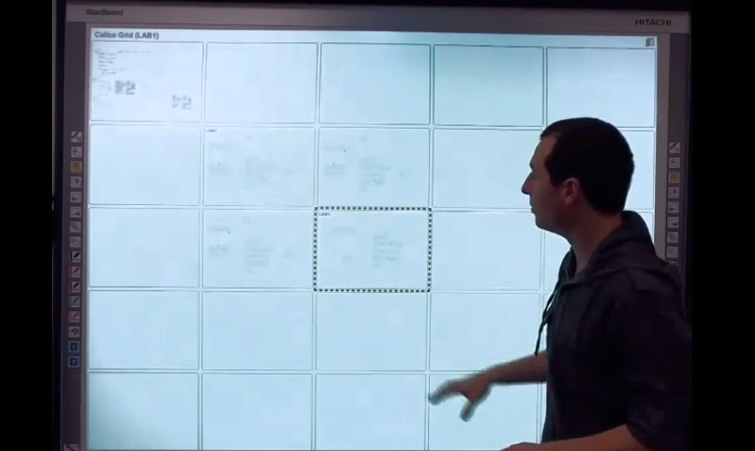
\includegraphics[width=0.8\textwidth]{grid.jpg}
\caption{The grid view within Calico}
\label{fig:grid}
\end{figure}
The grid is the focal point of any session in Calico.
It shows the various canvases that users may interact with in a given session.
Users may perform various operations on canvases from the grid, such as duplicating or clearing individual cells.
The grid also gives a clear overview of the designs that are happening in a session.

\section{Gestures}

\section{Scraps}
Scraps in Calico can be thought of as ``scraps of paper'' that one would place on a desk or on a white board.
Scraps can be easily relocated to different parts of the screen, or even other canvases.
Scraps can be stacked on top of each other and then treated as a unit or group.
By treating scraps as if they were pieces of paper, we [make it easy to understand the manipulation], as designers can easily relate Calico to their current design 

\section{Palette}
The palette in Calico provides users with a ``drawer'' that can easily be used to store commonly used shapes and artifacts.
The palette can be synchronized across sessions so that other users in the session can share the same palette.

\chapter{Objectives}

[old version was single user, list limitations] Calico was originally designed to be a single-user system that allowed individuals to operate an electronic whiteboard. While this original design worked great in an isolated environment, it made it very difficult for users to collaborate with one another. Users had to resort to taking screenshots and emailing them to one another.  Our aim with the new version of Calico was to create a system that would function in an isolated environment, but could easily facilitate collaboration with multiple users when needed. By designing with collaboration in mind, we were able to create a client-server architecture that would support many users interacting with the same canvas area simultaneously. The server had to be responsible for maintaining order of objects, as well as acting as a version control to make sure that users were not able to perform conflicting actions that would corrupt the drawings.

As an experiment, we worked to add collaboration to the original Calico implementation. This was able to help us determine that using Calico in a multi-user environment would be much more useful than we originally expected, and drove us to create a more robust multi-user implementation. Our attempts to [make old calico multi-user] were not successful, as the system was extremely sluggish and frustrated many users. We found that our users expected the system to be much more responsive, and the sluggishness was not acceptable. This was one of the biggest reasons that we decided to redesign a new Calico from the ground up.  

[reasoning for new iteration, rethinking architecture]Rather than continue working on the existing version of Calico, we discussed the [usefulness?] of redesigning the architecture from the ground up in order to better support the features we were hoping to add. We wanted to create a system based on the client-server architecture that would facilitate many clients all interacting with the system at the same time. The old version of Calico used a peer-to-peer connection that limited the number of active clients that could use the system. The old peer-to-peer architecture proved to be highly problematic when connecting with users over the Internet. While the system was able to work fine locally, the ultimate goal for the system was to collaborate with users all over the world, and we realized that a peer-to-peer architecture would not be ideal when collaborating over the Internet. This was one of the reasons we chose to move to a client-server architecture. We were able to place the server on a system that was open to the Internet, and it would eliminate all the connection problems that plagued the old peer-to-peer architecture. 

Another area where the client-server architecture benefitted us was with performance. We created a server that was highly optimized for processing data from many different clients at the same time. This allowed us to handle many more clients without any noticeable drop in processing time. Previous versions of Calico had the clients act as servers, which meant that in addition to processing all of the graphical data, they were also responsible for processing all incoming data and drawing what the other clients were sending.
[list requirements and wants/needs]
[req:distributed]
[req:persistence]The first iteration of Calico was a peer-to-peer system. This meant that there was no single place where the drawings would be stored. There was no way to view the contents of the session unless you were actively viewing it from within the Calico program itself. We wanted to be able to access the current state of a session without the need to actually join the session itself. By creating a central server that was responsible for maintaining the session, we were able to have a persistent history of the session. Users could join and disconnect, and then return, and still be able to undo operations that were performed long ago. Users could import canvas drawings into other programs by requesting a rendered image from the server. By storing the session state at a single location, we reduced the likelihood that data would become corrupted in transit, or data that would be corrupted synchronizing between many "master" servers as it had in the traditional peer-to-peer architecture. The persistent server was regarded as the true master, and if any client differed, it would synchronize with the central server, rather than assuming its own state was the "correct" version.

[req:sessions]Sessions was not initially planned in our rewrite of Calico, but we soon found a need for sessions to be added. The previous version of Calico had no session system at all, however it was not really necessary because users could essentially create their own sessions by just starting another instance of the program. This provided an easy method for users to work on various projects without interfering with the designs of another project. With the new client-server architecture, it was more difficult to start a new instance of the server in order to work on a separate project. Thus the need for sessions was realized, as designers needed a way to easily create a separate Calico instance that would not interfere with the existing session. 

[req:admin interface]One of the benefits of having a central server was the ability to have an "administrative interface" that could allow users to perform actions on the server, and backup/restore sessions. With the new version of Calico, we opted to create a web-based administrative interface that let the user perform various low-level commands that were used for debugging. Along with the ability to perform commands, users could download a file containing the entire state of a session. These files could then be restored at a later point in time, and would restore the session to its previous state. This proved to be very useful during the initial development, as it provided a safety net for users. Users were able to experiment more knowing they had a backup of their designs.


\chapter{High-Level Architecture}

Calico's new architecture was motivated by the design decisions listed below. 
The key design decisions for the new version of Calico were:

\begin{itemize}\itemsep1pt
  \item Client/Server architecture for improved connectivity over the Internet.
  \item Optimization of network traffic to reduce lag on distant clients, as well as network usage.
  \item A plugin framework to enable developers to create extensions into the Calico system.
  \item Improvement of input event handling system to improve drawing performance and input recognition.
  \item Consistency handling and persistence improvements to ensure that clients are all kept in the same state.
\end{itemize}

In the following sections, each decision will be explained in more detail.



\section{Client/Server Architecture}
We decided that the architecture needed to be redesigned in order to support all the planned changes. The new architecture that was chosen had to be able to support all the features, as well as easily support multiple users simultaneously. It also had to be accessible from anywhere, and had to be more stable than previous versions that were known to crash.

\begin{figure}[h]
\centering
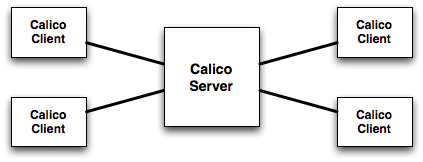
\includegraphics[width=0.8\textwidth]{arch_diag.png}
\caption{Overview of Calico's Architecture}
\label{fig:calico_arch}
\end{figure}

The first change made was a switch from the original peer-to-peer system to a completely new client-server architecture. We believed that by using a client-server architecture, we could provide a centrally accessible service that would easily support multiple clients and still maintain stability. The server could act as a headless service that could be more efficient since it did not have to perform any client functions such as rendering the display. This meant that the server could be dedicated to the task of managing all the interactions between clients, and could be much more stable than in a peer-to-peer context. When using peer-to-peer, each client was responsible for notifying all connected clients (which caused a large amount of network traffic). By switching to client-server, clients are only communicating with a single server, which greatly reduced the network traffic, and increased the stability of the network.

\section{Networking Component Overhaul}
One of the significant changes from the original Calico was the change in network communication design. The previous version of Calico had networking that was designed as an add-on at a later time, and was not fully integrated into the system. In this old design, when a change was made by another client, the entire change was saved to a Java object. This object was then serialized and sent in full over the network. The receiving client would deserialize this data, and then perform the change on its local drawing canvas. This process was very easy to implement, but had the cost of requiring significant processor time due to the constant serialization/deserialization process that would take place for each action. It also incurred the network overhead of Java serialization, which would add much more data to the final packet. All of this overhead would quickly become apparent to users when the system would lag in response to many actions done in quick succession. Our goal was to streamline this process as much as possible so that we could reduce lag when the system was being heavily utilized.

To improve the responsiveness of Calico, and reduce the network overhead, we created a custom packet design that could be used by Calico to notify both the client and server when various actions were performed. These special packets provided exactly what was needed to effectively communicate changes to clients, and thereby significantly reduced in size compared to the original design. Packets now are byte arrays that are written directly to the wire and, based on the format expected by the given command, are decoded back into their specific components (integers, strings, booleans, and floats). 



\begin{figure}[h!]
  \centering
  \begin{bytefield}{34}
    \bitbox{4}{length} & \bitbox{8}{command ID} & \bitbox{24}{command-specific data}
  \end{bytefield}
  \caption{A Calico network packet}
\label{fig:calico_packet}
\end{figure}

This packet design was loosely based on the packet design of the Half-Life game engine \cite{rcon}. As seen in the figure above, the packet is broken up into three main parts. The first four bytes of the packet is the length of the packet. This tells the network system how much farther it needs to read to ensure it receives the entire packet. The next four bytes hold the command identifier. This number is used to tell the network system what this packet is about. Both the client and the server have a list of commands and their IDs, which are used to translate from a programmer-friendly command name to the command ID number. The remaining bytes vary based on the specific command that is being transmitted. Each command has different parameters, of which both the client and server are aware. By writing data directly to the wire, there is little overhead -- each packet is as small as it could be. This makes the network communication between the client and server much more efficient, and helps to reduce the lag, even when put under heavy usage.

\section{Improvement of Input Handling System}
In the previous version of Calico, the input system was plagued by sluggish performance and inaccuracy. When there were many elements on the screen, the input system would lag and would begin to ``miss'' input data, which would result in straight lines instead of smooth curves. As a sketching tool, the ability to receive accurate input from the user was very important to the performance of the tool. The previous version of Calico routed input data directly to the rendering system, which would draw the images on screen. This made development very easy, but it required the input system to wait on the rendering process. This meant that the more images that had to be rendered, the longer the input system had to wait before it could start processing new input data. In Java, the mouse input listener does not queue input events -- if a program is too busy to receive input, then that input event is lost forever. Due to this problem, fluid drawing was nearly impossible.   

The new version of Calico is designed to fix this problem. By creating a separate, but dedicated input handling system, Calico can readily process input commands without having to wait for the rendering process to complete.

Instead of linking the input, action processing, and rendering systems serially, they are now linked in ``parallel'' using a multi-threaded approach. None of the separate processes are reliant on any of the other processes to complete, so input can be quickly received and queued if needed. These input events are then sent to the action processing system which determines what actions (if any) should be performed based upon the given input. Once an action is decided, the rendering process is notified and redraws the screen as needed. By using these components in parallel, we are able to remove the perceived lag and missed mouse events that would cause distortion and incorrect sketching. Even though the display can lag slightly behind the rendering system, this delay is not nearly as noticeable as when input events were being missed. 


\section{Consistency Handling / Persistence}
The previous version of Calico had many problems maintaining consistency between all clients. Clients would quickly become outdated and their states would not be consistent with that of the other clients. 
This problem was generally a result of parallel edits being performed. Clients would perform the edits locally, and then notify the other clients of the change. Often, the events would be received in a different order than they were being performed on a client, and the elements would be modified incorrectly. This led to identical elements being displayed very differently on multiple clients, due to the fact that there was no authority to resolve disputes when edits were being done to an element at the same time.
The previous version of Calico had no central server to check or update consistency, so any time where a client became inconsistent, designers had to quit the program and reconnect in order to fix the problem.
Naturally, this was very frustrating to users as it made it very difficult to collaborate with another user once the data became inconsistent. 

In the new version of Calico, this problem is fixed by implementing a system for checking and maintaining consistency across all clients connected to the server. In the new Calico, the server is considered to be the master, and all clients defer to the server to determine what state they should be at. All client actions are sent to the server and are not processed on the client until the server acknowledges the command. This means that all clients are given the same commands to modify elements at the same time. Clients are essentially ``unintelligent'' and do not assume any knowledge of where elements should be positioned -- this is all maintained by the server. This means that clients never become inconsistent, as there is a single system that is responsible for maintaining the state on each client system. 
Even when clients are editing the same element in parallel, Calico is able to maintain consistency by giving priority to the first event received. This allows users to edit the same element, and prevents the system from trying to issue conflicting edits to the same object.

The only time when clients now lose consistency was during network errors where packet loss is experienced. However, even if this were to occur, there are regular consistency checks that quickly realize the inconsistencies and fix them, without ever interrupting the designer. This system periodically notifies all clients of the current state of the system by sending a hash code to all clients. The hash code represents a checksum of the system and all of the drawing content. If any of the clients responds with a different hash code, they are sent an export of the entire session containing all the data needed to recreate the canvas from scratch. Because of this, any inconsistencies could easily be mitigated with minimal inconvenience to the end user. This meant that a session using the new version of Calico could last for weeks without problem -- something that was not possible in the previous version of Calico. The only drawback with this new process is that sometimes content changes unexpectedly for the user when parallel changes or packet loss occurs. While this is disruptive, the frequency of this occurring is low.


% Implementation (broken into sections)
\chapter{Implementation}
Maybe talk about the actual technical implementation?
\section{Networking}

\begin{figure}[htb]
  \centering
  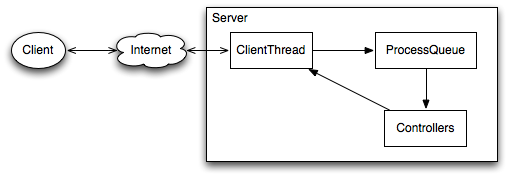
\includegraphics[width=0.8\textwidth]{network.png}
  \caption{Overview of Network Flow in Calico}
  \label{fig:network}
\end{figure}
% Intro parts
As a distributed and collaborative system, networking is a key part of Calico. The networking system must be able to support many clients at the same time, some of which may be working on the same canvas. The networking system in Calico consists of three major components: the main server socket and individual client process threads, the network queue processor, and the \texttt{CalicoPacket}. These three components work together to ensure that client requests are quickly handled, and that conflicts are properly managed.

% Socket/ClientThreads
The first component is the primary server socket and client threads. We decided to implement Calico as a TCP \cite{network} server in order to benefit from TCP's flow control and error correction. While TCP may be slower than UDP, the benefits of ensuring packets are received in the order they are sent as well as maintaining a continuous session outweighted any performance gains of UDP. When the Calico server is started, a TCP socket listener is created that waits for client connections to arrive. Upon receiving a new connection from a client, a new \texttt{ClientThread} is created that will then handle the connection with the client for the remainder of the client's session. By using a multi-threaded network system, we can easily maintain multiple sessions at the same time.

% ProcessQueue
The second component is the network queue processor, implemented as \texttt{ProcessQueue} class. This class is responsible for processing each packet that arrives from a client. When one of the \texttt{ClientThread}s receives a packet, the packet is then routed to the \texttt{ProcessQueue} which has a method for each packet type that can process that specific command. This class can then call any controllers as needed in order to complete the requested command.

% CalicoPacket
The \texttt{CalicoPacket} is responsible for encoding all information of a specific command into a byte array that can then be sent to clients. The packet is the lowest level of the networking system, but one of the most important. As noted in the previous section, the Calico packet was heavily based on Half-Life's network packet design. The first part of the packet contains a four-byte length which tells the system how far it needs to read in order to obtain the entire packet. By breaking commands down and transmitting them at the byte level, we were able to greatly reduce the network overhead that would be created if we had decided to send serialized objects over the network instead.

\begin{figure}[h!]
  \centering
  \begin{bytefield}[bitwidth=0.9em]{33}
    \bitbox{5}{command} 
    & \bitbox{4}{uuid} 
    & \bitbox{4}{cuid} 
    & \bitbox{4}{puid} 
    & \bitbox{2}{r} 
    & \bitbox{2}{g} 
    & \bitbox{2}{b} 
    & \bitbox{4}{points} 
    & \bitbox{2}{x1}
    & \bitbox{2}{y1}
    & \bitbox{2}{x2}
    & \bitbox{2}{y2}
    \\
    \bitbox{5}{230} 
    & \bitbox{4}{100} 
    & \bitbox{4}{1} 
    & \bitbox{4}{0} 
    & \bitbox{2}{255} 
    & \bitbox{2}{0} 
    & \bitbox{2}{0} 
    & \bitbox{4}{2} 
    & \bitbox{2}{0}
    & \bitbox{2}{0}
    & \bitbox{2}{2}
    & \bitbox{2}{2}
  \end{bytefield}
  \caption{An example STROKE\_LOAD packet}
\label{fig:stroke_packet}
\end{figure}


As an example, say a client has connected to the server for the first time. As soon as they join the server, the server will begin to notify them about all the elements that are visible on all canvases. An example of this would be the \texttt{STROKE\_LOAD} command which is used to notify a client about a stroke element. To notify the client, the server must create a \texttt{CalicoPacket} that can be sent to the client. The first part of the packet is the command ID. In this case, the command ID for \texttt{STROKE\_LOAD} is 230. The second, third, and fourth values are 64-bit integers used to denote the stroke's UUID, the UUID of the canvas that it belongs to, and the UUID of its parent element, respectively. The next three values are 32-bit integers used to denote the red, green, and blue values of the stroke's color. The next value is a 32-bit integer that indicates how many coordinates are used to describe the ``path'' of this stroke element. The remaining values are the actual coordinates used to describe the path. They are listed in x,y-pairs. A graphical version of this packet can be seen in Figure \ref{fig:stroke_packet}. This describes the logic required to generate a single \texttt{STROKE\_LOAD} command. 

\section{Object Storage}
In Calico, all core components are stored using high performance Java hash maps. 
We decided that using FastUtil's \cite{fastutil} high performance maps would provide a better response time as opposed to using Java's core HashMap class. 
Each controller contains a single hash map that acts as a database for all objects that the controller is responsible for.
All access to hash maps requires use of a ``key'' to perform a lookup.
All objects are given a sequential 64-bit integer that acts as a globally unique identifier for each object.

One important design decision that was made was the choice to use a sequential identifier for each new object. The two factors that influenced our decision were: the relatively small size of a 64-bit integer in comparison with a universally unique string (which would be almost double the size), and better client performance.
Small size was very important to us as this identifier is included in nearly every network packet that is sent to and from the server. We wanted the footprint to be as small as possible, but we needed something that we could ensure would be unique for every object. 
The second decision -- better client performance -- was another benefit provided by using a sequential identifier. Clients can request a pre-allocated block of identifiers that they can assign to objects created client-side. The client can then create objects and assign them an identifier and submit the object directly to the server. Due to the fact that identifiers are pre-allocated, the client does not have to wait for confirmation from the server in order to add the object to its local hash map.


\begin{figure}[h!]
  \centering
  \begin{subfigure}[t]{0.4\textwidth}
    \centering
    \small
    \verbatiminput{figures/java/storage_stroke.java}
    \normalsize
    \caption{Stroke}
    \label{code:stroke_storage}
  \end{subfigure}%
  ~ 
  \begin{subfigure}[t]{0.4\textwidth}
    \centering
    \small
    \verbatiminput{figures/java/storage_scrap.java}
    \normalsize
    \caption{Scrap}
    \label{code:scrap_storage}
  \end{subfigure}
  \caption{Calico object representations}
  \label{code:storage}
\end{figure}

Figure \ref{code:storage} shows snippets from two objects within Calico. The first is the \texttt{Stroke} element (which provides lines) and second is the \texttt{Scrap} object. A graphical depiction of scraps can be seen in Figure \ref{fig:scraps_storage} as the light gray areas. Scraps can be parented within other scraps (if a scrap is completely contained within another scrap, then the larger scrap would be considered the parent of the smaller scrap).

Figure \ref{code:storage} shows how all elements within Calico are provided with a unique 64-bit \texttt{uuid} which acts as the ID for the object. The second field, \texttt{parentUUID} is the ID value of the parent object that contains the current object. If the current object is not parented, then this would be set to \texttt{0L}. The third field is the \texttt{canvasUUID}. This value is always present, as it links the current element to the specific canvas that it was created on. Every element within Calico must be created on an existing canvas. 

The last field that is shared among Calico elements is the \texttt{points} field. We decided to use Java's native \texttt{Polygon} class to represent the coordinate path of the given element. By using a \texttt{Polygon} object, we are able to use native geometry operations to determine containment and intersection of elements. When a stroke is being drawn on a client machine, the server will continously append \texttt{Point2D} objects to the \texttt{points} field for the respective Stroke. 

The \texttt{Scrap} class shown in Figure \ref{code:scrap_storage} also includes three additional sets: \texttt{childScraps}, \texttt{childStrokes}, \texttt{childArrows}. These sets contain a list of UUIDs that can be mapped to any element that is a child of this scrap. These sets are accessed whenever a parent scrap is deleted or moved, because all operations must be executed on all child elements.


\begin{figure}[h!]
  \centering
  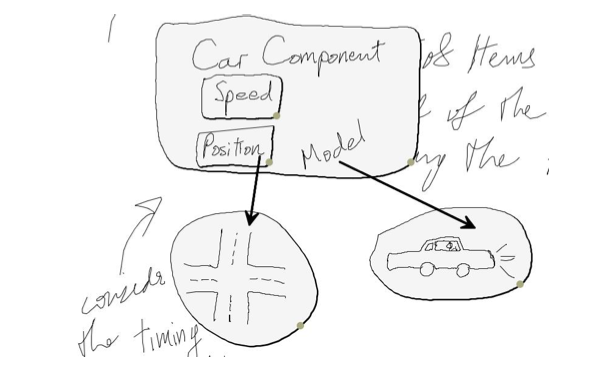
\includegraphics[width=0.8\textwidth]{scraps.png}
  \caption{Calico design session}
  \label{fig:scraps_storage}
\end{figure}

The screenshot shown in Figure \ref{fig:scraps_storage} displays a typical design session in Calico. This image represents a single \texttt{Canvas} object which would be stored within the \texttt{CanvasController} class. The \texttt{Canvas} object would have a list that contains the identifiers for each object that is being displayed on screen (five \texttt{Scrap}s, two \texttt{Arrow}s, and many \texttt{Stroke}s). Each of these objects is stored in their respective controller. Each of these objects requires a list of \texttt{Point}s that form the boundaries of the object. These are used within Calico to determine the location of an object, as well as whether an object is contained within another object (such as a scrap). Each object can have additional attributes that are specific to its type (arrows need endpoints, strokes have a color). These attributes are stored within the object itself and are converted to a \texttt{CalicoPacket} whenever a new client connects and needs to load the existing state of Calico.




\section{Object Controllers}
In Calico, object controllers are responsible for handling all operations made on elements under their control. Each object type in Calico is provided with a controller.
Scraps, strokes, arrows, and canvases each have a controller that handles any interaction performed on the object. 
Controllers also act as the storage points for the objects they are responsible for, as discussed in the previous section.

Controllers are created as static classes. This means that each method in the controller always is provided with the object's identifier, which it can then use to locate the object within the database. 
The controllers are also responsible for notifying the server of any changes that are performed. However, in order to prevent clients from sending notifications for actions that were not performed by the user, we created two types of functions for each action in the controller. The first function performs the action and then notifies the server, while a second function performs the action without sending notifications. Any operation that was performed by the user will lead to a notification sent to the server. Any operation that was the result of receiving input from the server will not send a notification.

\begin{figure}[htb]
  \centering
  \small
  \verbatiminput{figures/java/controller.java}
  \normalsize
  \caption{Partial source of Calico's Stroke Controller}
  \label{code:controller}
\end{figure}
% class StrokeController {
%   public static void start(long uuid, long cuid, long puid, Color color);
%   public static void append(long uuid, int x, int y);
%   public static void finish(long uuid);
%   public static void delete(long uuid);
%   public static void move(long uuid, int deltaX, int deltaY);
% }

Figure \ref{code:controller} shown above provides an excerpt of code from one of Calico's controllers. This example shows the basic operations that are available for the \texttt{StrokeController}. This controller is responsible for handling all ``stroke'' elements (line drawings). The controller is designed to be a globally available backend that can be accessed by both the network connection (so that strokes can be created by the server) as well as by the input system (so strokes can be created using mouse events). 

Imagine the following scenario that we will use to describe how the Calico client would normally interact with the controller to create a sketched line on screen. In our example, we start with a blank \texttt{Canvas} screen, ready to begin sketching. The first event would be a \texttt{MouseEvent.MOUSE\_PRESSED} event that is sent to Calico's input handlers. The input handlers are responsible for ensuring that the user is in the proper mode (for sketching) and that the user is not clicking on a button. Once the input handler has determined that the user intends to sketch on screen, the event is handed off to the controller.

We first need to extract the \texttt{x} and \texttt{y} positions of the mouse coordinates from the \texttt{MouseInputEvent} object. The next step would be to obtain a new \texttt{uuid} for our stroke. This requires a call to \texttt{Calico.uuid()} which provides us with a new 64-bit integer that is unique across all clients. We now have all the information needed to start our stroke element, so execute a call to \texttt{StrokeController.start(uuid, canvasUUID, 0L, Color.RED)}. This creates a new stroke that is colored red, and has the provided \texttt{uuid}. 

Our stroke has been started, but at this moment there are no coordinates attached to the stroke. We will next need to call \texttt{StrokeController.append(uuid, xPos, yPos)} using the \texttt{x} and \texttt{y} positions of the mouse that we extracted in the previous paragraph. The call to \texttt{append} will repeat for every \texttt{MouseEvent.MOUSE\_DRAGGED}, until the \texttt{MouseEvent.MOUSE\_RELEASED} event is fired.

When the mouse has been released, Calico will make a call to the \texttt{StrokeController. finish(uuid)} method which signals that the user has finished drawing the stroke element, and it should be finalized. During the \texttt{finish} method, it ensures that the stroke is properly parented (if it is contained within a scrap, it will be added to that scrap).

During this process explained above, the client is sending events to the server (\texttt{STROKE\_START}, \texttt{STROKE\_APPEND}, \texttt{STROKE\_FINISH}). When the server receives these events, it performs an identical set of controller calls to record the sketching server-side. It will also mirror these commands to all connected clients. The benefit to using a global controller on the client is that when a stroke (or any element) is created by another user, the \texttt{CalicoPacket} can be easily mapped to the proper controller methods.
\section{Plugin Framework}
To improve the extensibility of Calico, a plugin framework was created. This plugin framework allows for new features to be integrated into Calico without needing to directly modify its core code. Plugins subscribe to specific events that they want to be notified about. When one of these events is triggered by Calico, all subscribers to that event are notified, and can choose to perform any action based upon the event information. 

\begin{figure}[h!]
  \centering
  \small
  \verbatiminput{figures/plugin.java}
  \normalsize
  \caption{Example plugin source code}
  \label{code:plugin_file}
\end{figure}

To create a plugin, developers only have to extend a provided abstract plugin class that allows each plugin to register itself with a \texttt{PluginManager} that is responsible for publishing network events and interface events to each plugin (see Figure \ref{code:plugin_file}). Plugins were provided with default ``hooks'' that are called when the plugin is loaded or unloaded. Plugins call a method \texttt{registerNetworkCommandEvents} to subscribe to specific network commands that it was interested in. Another method, \texttt{RegisterPluginEvent}, enables the plugin to subscribe to various interface events that are used for processing user input and clicks. For instance, plug-ins can register to be notified when a scrap or stroke is created. When the server receives the \texttt{SCRAP\_FINISH} event, the plugin will immediately be notified about the scrap, and will be given the identifier corresponding to the scrap. With this information, the plugin can obtain the scrap from the database and can then perform further operations if needed. For example, a plugin can listen for newly created scraps and submit a screenshot of each scrap to a remote service as soon as the user creates the scrap.

\subsection*{Interaction with Core Elements}
We decided to allow plugins to access the core Calico controllers to be able to create, modify, and delete core elements (\texttt{Scrap}s, \texttt{Stroke}s, \texttt{Arrow}s). For example, we created a chat robot that would listen for incoming text messages, and upon receiving a message, creates a new \texttt{Scrap} with the given message as the contents. In another example, we created a plugin that generates an image based on the current canvas and submits this image to an outside service to be saved.

\subsection*{Restrictions}
While plugins were given a great amount of freedom when it came to interacting with the core elements, they are not allowed to modify Calico's interface. Plugins in particular can not create custom versions of \texttt{Scrap} elements or \texttt{Stroke} elements. We decided that we did not want to allow that flexibility. Instead, plugins are given just the freedom to manipulate elements, but not customize them further. Additionally, plugins are not allowed to customize the global interface of Calico -- they are not allowed to add buttons or change the layout of the menus. Again, these were not features we thought necessary for the level of customization that plugins were designed for.
\section{Input Handling}
% - talk about input handling system (how i know what object you touch)
% when the mouse pressed, locate all scraps that contain the mouse location
% determine the smallest scrap that contains the location
% actions are performed on that
% input handler is then "locked" onto that specific group (so that during the move, we are not trying to calculate over and over)
% unlocked as soon as it is released
% each object knows the list of points (or path) that acts as its bounds.
% Each object can then know if a specific point is within
In an effort to improve the user interaction experience, we felt that the existing input handling system needed to be created specifically for Calico. The previous version of Calico had relied on the input handler provided by the drawing framework that was used. This became unusable when working with canvases containing hundreds of objects. To improve response times, we need to recreate a newer input handler that did not rely on the drawing framework - meaning that it could continue to operate even while the drawing framework was busy rendering the display.

Rather than having a specific mouse listener linked to each object on screen, we instead decided to have a global mouse listener that could determine which object was being touched. This meant that mouse input only needed to be processed by a single handler, and based on various modes, it could intelligently handle interaction with the user. 

Each canvas maintained a list of all objects that were present on screen. Each object also was responsible for maintaining a list of coordinates that formed the ``bounds'' of that object. Objects could then easily determine if a specific point was contained with the ``bounds'' of that element.
Upon receiving any mouse input, the input handler would then iterate through the elements and determine which elements contained the mouse location. This list would then be further reduced to return only the \emph{smallest} object that contained the mouse location. This was very helpful when handling scraps that had been stacked on top of each other - the parent scrap still contains the mouse location, but clearly the user wants to interact with one of the child elements.

After locating the element that the user will be performing actions with, the input handler would then be ``locked'' to only interact with that element until the mouse has been released. This meant that users could move a scrap around screen (and move the mouse outside the bounds of the selected scrap) and still have the scrap follow the mouse location. Another benefit of locking the input handler on a specific element was that while doing very intensive operations (such as moving an element across the screen) we were not wasting resources to recalculate which element we were interacting with. This is something that was not availble in the previous versions of Calico.

The one drawback to using this approach meant that the object location and screen coordinate systems were identical. What that meant was that the Calico coordinate system was equal to the user's screen resolution. If a user with a larger screen joined the session, they could draw shapes and figures that were outside the viewable area of users with smaller screens. At the time, this was not a problem because all users were running the same resolution, so fortunately this problem rarely occurred.
\section{Administrative Interface}
% - admin web server
% uses httprequesthandlers
% velocity templates
% based off phpBB admin interface
% has a few basic functions, and allows admins to administer those
% view connected clients
% update configuration values
% upload images
% execute specific commands
% perform backup
% restore backups
One of the last components to be added was the administrative interface. Calico now had a headless server, and we needed a way to remotely manage it. We decided against building the interface within the Calico client - we wanted to keep the client as lightweight as possible. 
We decided to create an easy to use web-based interface that would allow the Calico server to be managed easily using a web browser.

The administrative interface only provided basic management abilities. The core abilities it provided were:
\begin{itemize}\itemsep1pt

\item
\textbf{Easily modify settings}.
We needed the ability to modify the settings of an existing Calico instance easily. What was created was a page that listed all the configuration variables and easily let the administrator modify those values. When saved, the Calico server could then be restarted if needed to reflect the configuration changes.

\item
\textbf{View currently connected clients}. 
This was helpful in the classroom environment to be able to see all users who were currently connected to the server. In the future we planned to add the ability to ``kick'' clients from the server, but this was never full developed.

\item
\textbf{Perform backups and restoration of sessions}.
One of the major requirements was the ability to easily generate a backup of an entire session. Our goal was to provide an easily way to download a backup file that represented the current state of the server. It needed to contain all the data required to fully restore all canvases and any scraps, strokes, or arrows that may be contained in the canvas. Once we created the backup system, we needed a way for a server to restore any backup. Our administrative interface provided an easy to use form where a backup file could be selected and then uploaded directly to a running server. The server would then read the contents of this file and import all data into the server. Restoring a backup essentially wiped any existing content and recreated the entire session from scratch. Once a restoration had been performed, clients could reconnect and they would see all the data, just as it was when the backup was created.

\end{itemize}

These few requirements were the driving force behind the administrative interface. It stands as a very barebones and minimalistic interface that provides functions that we decided were essential to operation. This administrative interface has proved invaluable when generating and restoring backups. Having a backup of sessions provides users with a greater level of reassurance that any work they have made will not be lost should anything happen to the server.

% list of website paths and each one is mapped to a request handler for that specific action
% 
To keep the admin system lightweight, we decided to utilize the \texttt{HttpComponents} library provided by the Apache Foundation\cite{apache:http}. This library provides a single webserver endpoint that will route all web requests to a predefined list of request handler endpoints. These endpoints are specified in the \texttt{AdminRequestListenerThread} class within Calico. The most important part of this request handler is the ``request registry''. This registry acts as a routing engine that will route requests made to certain endpoints to a specific request handler designed to handle that request.

\begin{figure}[h!]
  \centering
  \small
  \verbatiminput{figures/java/request_registry.java}
  \normalsize
  \caption{Administration interface routing example}
  \label{code:request_registry}
\end{figure}

In figure \ref{code:request_registry}, you can see a code snippet of the routing table. The important part is the call to \texttt{reqistry.register}. In this snippet, you can see that any requests that are sent to \texttt{/gui/config/} will be sent to the \texttt{ConfigIndexRH} class to be processed. This allowed us to break the administration system into logical components each designed to handle a different aspect of the server. 

\begin{figure}[h!]
  \centering
  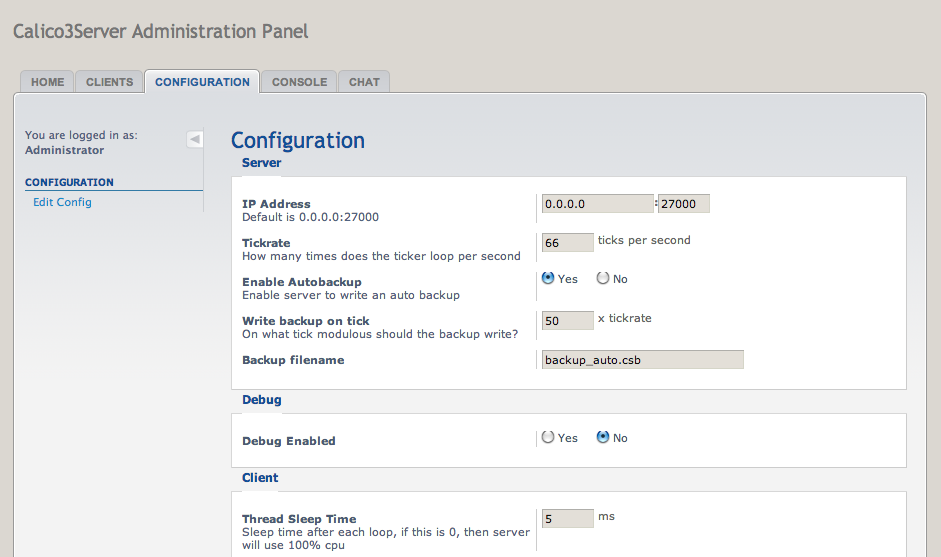
\includegraphics[width=0.9\textwidth]{admin_ui.png}
  \caption{Admin configuration form (/gui/config/)}
  \label{fig:admin_config}
\end{figure}

One example request handler would be the \texttt{ConfigIndexRH} class that was mentioned above. This class was responsible for two separate tasks. The first task was to process a \texttt{GET} request to \texttt{/gui/config/} which meant that the configuration form should be displayed in the user's browser (an example form can be seen in figure \ref{fig:admin_config}). To easily create the HTML required for the administration interface, we decided to use a templating framework that would allow us easily write HTML that contained placeholders that could be rendered by the request handlers. The template framework that we chose to use was Apache's Velocity\cite{velocity} framework. We decided to use Velocity because of its ease-of-use as well as its powerful language that allowed us to create various macros to easily abstract common interface elements. The interface look-and-feel was copied from the administrative interface of an open-source forum system known as PhpBB\cite{phpbb}. Figure \ref{code:tpl_config} shows a snippet of the template language that was used to generate the configuration form seen in figure \ref{fig:admin_config}.

\begin{figure}[h!]
  \centering
  \small
  \verbatiminput{figures/tpl/config.tpl}
  \normalsize
  \caption{Snippet of the Velocity template for configuration page}
  \label{code:tpl_config}
\end{figure}

The second task of the configuration request handler was to process a \texttt{POST} request to the same endpoint. This request was for a form submission, which instructed the server to update the configuration settings on the server to reflect the values entered in the configuration form.

\chapter{Conclusion}
In conclusion, Calico is awesome.

% These commands fix an odd problem in which the bibliography line
% of the Table of Contents shows the wrong page number.
\clearpage
\phantomsection

% plain
%\bibliographystyle{abbrv} % DEFAULT
\bibliographystyle{acm}
%\bibliographystyle{abbrvnat}
\bibliography{thesis}

\appendix

\section{Calico Network Commands}
\begin{table}[h]
  \begin{tabular}{ | l | l | }
  \hline
  \textbf{Command Name} & \textbf{Format} \\ 
  \hline
  JOIN & SS \\
  \hline
  HEARTBEAT & LI \\
  \hline
  GROUP\_START & LLLI \\
  \hline
  GROUP\_APPEND & Lii \\
  \hline
  GROUP\_MOVE & LII \\
  \hline
  GROUP\_DELETE & L \\
  \hline
  GROUP\_DROP & L \\
  \hline
  GROUP\_FINISH & LB \\
  \hline
  GROUP\_SET\_CHILDREN & LII \\
  \hline
  GROUP\_SET\_PARENT & LL \\
  \hline
  GROUP\_MOVE\_START & L \\
  \hline
  GROUP\_MOVE\_END & LII \\
  \hline
  GROUP\_SET\_PERM & LI \\
  \hline
  GROUP\_RECTIFY & L \\
  \hline
  GROUP\_CIRCLIFY & L \\
  \hline
  GROUP\_CHILDREN\_COLOR & LIII \\
  \hline
  GROUP\_RELOAD\_START & LLLI \\
  \hline
  GROUP\_RELOAD\_FINISH & L \\
  \hline
  GROUP\_RELOAD\_COORDS & LIII \\
  \hline
  GROUP\_RELOAD\_CHILDREN & LIL \\
  \hline
  GROUP\_RELOAD\_POSITION & LII \\
  \hline
  GROUP\_RELOAD\_REMOVE & L \\
  \hline
  GROUP\_DUPLICATE & L \\
  \hline
  GROUP\_APPEND\_CLUSTER & LiII \\
  \hline
  GROUP\_SET\_CHILD\_GROUPS & Li \\
  \hline
  GROUP\_SET\_CHILD\_STROKES & Li \\
  \hline
  GROUP\_SET\_CHILD\_ARROWS & Li \\
  \hline
  GROUP\_REQUEST\_HASH\_CHECK & L \\
  \hline
  GROUP\_LOAD & LLLBiIIBddd \\
  \hline
  GROUP\_HASH\_CHECK & Li \\
  \hline
  GROUP\_COPY\_TO\_CANVAS & LLLII \\
  \hline
  GROUP\_SET\_TEXT & LS \\
  \hline
  GROUP\_SHRINK\_TO\_CONTENTS & L \\
  \hline
  GROUP\_IMAGE\_DOWNLOAD & LLSII \\
  \hline
  GROUP\_IMAGE\_LOAD & LLLSIIIIBiII \\
  \hline
  GROUP\_ROTATE & Ld \\
  \hline
  GROUP\_SCALE & Ldd \\
  \hline
  GROUP\_CREATE\_TEXT\_GROUP & LLSII \\
  \hline
  GROUP\_MAKE\_RECTANGLE & LIIII \\
  \hline
  GRID\_SIZE & II \\
  \hline
  UUID\_BLOCK & ILL \\
  \hline
  \end{tabular}
\end{table}

\begin{table}[h]
  \begin{tabular}{ | l | l | }
  \hline
  \textbf{Command Name} & \textbf{Format} \\ 
  \hline
  CANVAS\_INFO & LSII \\
  \hline
  CANVAS\_UPDATE & L \\
  \hline
  CANVAS\_UNDO & L \\
  \hline
  CANVAS\_REDO & L \\
  \hline
  CANVAS\_RELOAD\_START & L \\
  \hline
  CANVAS\_RELOAD\_FINISH & L \\
  \hline
  CANVAS\_RELOAD\_STROKES & LIL \\
  \hline
  CANVAS\_RELOAD\_GROUPS & LIL \\
  \hline
  CANVAS\_RELOAD\_ARROWS & LIL \\
  \hline
  CANVAS\_CLEAR\_FOR\_SC & L \\
  \hline
  CANVAS\_SC\_FINISH & L \\
  \hline
  CANVAS\_LOCK & LBSL \\
  \hline
  STATUS\_MESSAGE & S \\
  \hline
  ERROR\_MESSAGE & S \\
  \hline
  ERROR\_POPUP & S \\
  \hline
  CLICK\_TRACK & I \\
  \hline
  BGE\_APPEND & LII \\
  \hline
  BGE\_COLOR & LIII \\
  \hline
  BGE\_COORDS & LIII \\
  \hline
  BGE\_DELETE & L \\
  \hline
  BGE\_FINISH & L \\
  \hline
  BGE\_MOVE & LII \\
  \hline
  BGE\_START & LLL \\
  \hline
  BGE\_PARENT & LL \\
  \hline
  BGE\_CONSISTENCY & L \\
  \hline
  BGE\_RELOAD\_START & LLLIII \\
  \hline
  BGE\_RELOAD\_COORDS & LIII \\
  \hline
  BGE\_RELOAD\_FINISH & L \\
  \hline
  \end{tabular}
\end{table}

\begin{table}[h]
  \begin{tabular}{ | l | l | }
  \hline
  \textbf{Command Name} & \textbf{Format} \\ 
  \hline
  STROKE\_RELOAD\_START & LLLIII \\
  \hline
  STROKE\_RELOAD\_COORDS & LIII \\
  \hline
  STROKE\_RELOAD\_FINISH & L \\
  \hline
  STROKE\_RELOAD\_REMOVE & L \\
  \hline
  STROKE\_RELOAD\_POSITION & LII \\
  \hline

  STROKE\_START & LLLIII \\
  \hline
  STROKE\_APPEND & LiII \\
  \hline
  STROKE\_FINISH & L \\
  \hline
  STROKE\_SET\_COLOR & LIII \\
  \hline
  STROKE\_SET\_PARENT & LL \\
  \hline
  STROKE\_MOVE & LII \\
  \hline
  STROKE\_DELETE & L \\
  \hline
  STROKE\_LOAD & LLLCidddII \\
  \hline
  STROKE\_HASH\_CHECK & L \\
  \hline
  STROKE\_MAKE\_SCRAP & LL \\
  \hline
  STROKE\_MAKE\_SHRUNK\_SCRAP & LL \\
  \hline
  STROKE\_DELETE\_AREA & LL \\
  \hline
  STROKE\_ROTATE & Ld \\
  \hline
  STROKE\_SCALE & Ldd \\
  \hline
  STROKE\_SET\_AS\_POINTER & L \\
  \hline
  STROKE\_HIDE & LB \\
  \hline
  STROKE\_UNHIDE & L \\
  \hline

  ERASE\_START & L \\
  \hline
  ERASE\_END & LB \\
  \hline

  PLUGIN\_EVENT & S \\
  \hline



  CONSISTENCY\_CHECK &  \\
  \hline
  CONSISTENCY\_FINISH &  \\
  \hline
  CONSISTENCY\_CHECK\_CONTINUE & L \\
  \hline
  CONSISTENCY\_FAILED &  \\
  \hline
  CONSISTENCY\_RESYNC\_CANVAS & L \\
  \hline


  ARROW\_CREATE & LLICILIIILII \\
  \hline
  ARROW\_DELETE & L \\
  \hline
  ARROW\_SET\_TYPE & LI \\
  \hline
  ARROW\_SET\_COLOR & LIII \\
  \hline


  BACKUP\_FILE\_INFO & L \\
  \hline
  BACKUP\_FILE\_START &  \\
  \hline
  BACKUP\_FILE\_END &  \\
  \hline
  BACKUP\_FILE\_ATTR & SS \\
  \hline

  LIST\_CREATE & LLLLI \\
  \hline
  LIST\_LOAD & LLLBiII \\
  \hline
  LIST\_CHECK\_SET & LLLLB \\
  \hline
  \end{tabular}
\end{table}

Formats:
S-string. s-short. C-color. c-char. L-long. I-signed integer. i-unsigned integer. B-boolean. b-byte. f-float. d-double


\end{document}
